% "Outcome Bias in AI Models ..." -- version for The Aeronautical Journal (Royal Aeronautical Society / Cambridge University Press),
% in the journal's own LaTeX class (aer.cls, from the journal's template files, supplied by the author on 4 November 2026).
% Single-anonymised review, so the author is named. APA author-year references, as Cambridge's "Preparing your materials" page asks
% (the template's sample shows the older numbered style). Text as in the previous version of this file (checked against the preprint),
% with its prose revised for style on 11 November 2026 (lists and run-in labels turned into paragraphs; no number, finding or hedge changed);
% the metadata commands are left empty, as the template's guide asks. Build: latexmk -pdf paper.tex
\documentclass{aer}
\usepackage{txfonts}
\usepackage{longtable,booktabs,array,calc}
\usepackage{etoolbox}
\AtBeginEnvironment{longtable}{\footnotesize\linespread{1}\selectfont}
\usepackage{lineno}
\usepackage{xurl}
\usepackage[hidelinks]{hyperref}
\DeclareUnicodeCharacter{2212}{\ensuremath{-}}
\DeclareUnicodeCharacter{00D7}{\ensuremath{\times}}
\DeclareUnicodeCharacter{2260}{\ensuremath{\neq}}
\providecommand{\tightlist}{\setlength{\itemsep}{0pt}\setlength{\parskip}{0pt}}
\setlength{\emergencystretch}{2em}

\jmonth{}
\jyear{}
\volume{}
\issue{}
\historydate{}
\doi{}

\begin{document}

\markboth{Le Cuirot}{Outcome bias in AI models applying a culpability decision tree}

\title{Outcome Bias in AI Models Applying a Culpability Decision Tree to Airline Occurrence Reports}
\subtitle{A Pre-registered Within-Case Experiment}

\author{J. Le Cuirot\email{james@citadelaero.com}}
\affil{CitadelAero\\ Jersey\\ Channel Islands}

\maketitle

\begin{abstract}
Just culture judges people on what they knew and did, regardless of how events turned out. As AI models begin to code safety reports, this pre-registered within-case experiment tested whether they judge identical crew actions as more culpable when an occurrence ends badly. Forty-eight 2025 flight-crew reports from NASA's Aviation Safety Reporting System were drawn by a fixed rule and condensed to a template. Each case had two versions that differed only in the outcome, either the safe ending as reported or a fixed, plausible bad ending with minor injuries. Claude Sonnet 5.5, GPT-6.1 Sol and DeepSeek V4 Pro applied Reason's culpability decision tree to each version independently, under two prompt wordings, five times each (2,880 calls, plus 360 on controls), and the outcome was derived in code from their yes/no answers. All three models reached more culpable outcomes after a bad ending, with mean shifts of +0.35 (Claude), +0.25 (DeepSeek) and +0.18 (GPT) steps on Reason's nine-step scale (Holm-adjusted p = .0009, .007, .023); 14--18 of 48 cases were judged more harshly and 2--3 more leniently. For Claude and GPT the shift entered mainly through the substitution test, and for DeepSeek also through judgements that the crew knowingly violated procedures. Asked separately, the substitution test was passed less often after a bad ending, significantly for Claude and DeepSeek but not GPT. Control cases were unaffected. Models gave the same outcome on all five repeats in only 72--82\% of cells. A structured just-culture instrument did not prevent outcome bias.
\end{abstract}


\section*{NOMENCLATURE}
\begin{deflist}
\listterm{\emph{ACN}}{ASRS accession number (report identifier)}
\listterm{\emph{AI}}{artificial intelligence}
\listterm{\emph{API}}{application programming interface}
\listterm{\emph{ASRS}}{Aviation Safety Reporting System (NASA)}
\listterm{\emph{ATC}}{air traffic control}
\listterm{\emph{CC BY}}{Creative Commons Attribution licence}
\listterm{\emph{CI}}{confidence interval}
\listterm{\emph{D1--D11}}{deviations from the registered plan (Appendix C)}
\listterm{\emph{EU}}{European Union}
\listterm{\emph{FAR}}{Federal Aviation Regulations (US)}
\listterm{\emph{GAIN}}{Global Aviation Information Network}
\listterm{\emph{H1--H3}}{pre-registered hypotheses}
\listterm{\emph{HTTP}}{Hypertext Transfer Protocol (status 429: too many requests)}
\listterm{\emph{ID}}{identifier}
\listterm{\emph{JSON}}{JavaScript Object Notation (the reply format)}
\listterm{\emph{LLM}}{large language model}
\listterm{\emph{NASA}}{National Aeronautics and Space Administration (US)}
\listterm{\emph{OSF}}{Open Science Framework}
\listterm{p}{two-sided $p$ value (Holm-adjusted where stated)}
\listterm{\emph{Q1--Q5}}{questions of Reason's culpability decision tree, with sub-questions Q1b--Q4b}
\listterm{r}{Pearson correlation coefficient}
\listterm{\emph{RA}}{resolution advisory (TCAS)}
\listterm{\emph{S08}}{case identifier (main case 8)}
\listterm{\emph{SHA-256}}{Secure Hash Algorithm, 256-bit (file fingerprint)}
\listterm{\emph{TCAS}}{Traffic Alert and Collision Avoidance System}
\listterm{\emph{US}}{United States}
\listterm{\emph{USD}}{United States dollars}
\listterm{\emph{W1, W2}}{the two prompt wordings (investigator and neutral framing)}
\listterm{$W^{+}$}{Wilcoxon signed-rank statistic (sum of positive ranks)}
\listterm{z}{standard normal test statistic}
\end{deflist}

\subsection*{Greek Symbol}
\begin{deflist}
\listterm{$\kappa$}{Fleiss' kappa}
\end{deflist}

\linenumbers

\hypertarget{introduction}{%
\section{INTRODUCTION}\label{introduction}}

Aviation's reporting systems depend on a promise that a crew who report an error made in good faith will not be punished for it, provided the error is ``commensurate with their experience and training''. Gross negligence, wilful violations and destructive acts remain out of bounds. European law writes that promise into its definition of \emph{just culture} (Regulation (EU) No 376/2014, Art. 2(12)), and knowing the outcome of an occurrence is a well-known threat to it.

Decades of research show that people judge the same decision as worse, and the same person as more to blame, when the outcome is bad. The effect has been found in decision evaluation generally (Baron \& Hershey, 1988) and in hindsight estimates of what ``should have been'' foreseen (Fischhoff, 1975). It appears in physicians' judgements of the appropriateness of care (Caplan, Posner \& Cheney, 1991), in legal judgements of negligence and blame (Kneer \& Skoczeń, 2023), and among pilots evaluating other pilots' weather decisions (Walmsley \& Gilbey, 2016). Just-culture guidance exists largely to counter this tendency (Dekker, 2007), and hindsight is recognised as a barrier to learning from adverse events (Henriksen \& Kaplan, 2003).

Reason's (1997, p.~209) culpability decision tree is a well-known tool for this purpose. Its yes/no questions ask, in sequence, whether the actions and consequences were intended, whether a substance or medical condition was involved, and whether the person knowingly violated workable procedures. They go on to ask whether a comparable peer would probably have done the same (the substitution test) and whether there is a history of unsafe acts. None of the questions mentions the outcome, and a tree applied as designed should return the same answer for the same acts, whatever happened afterwards.

AI, meanwhile, is moving into safety departments' own work. A recent systematic review of AI for aviation safety found accident analysis to be the largest single topic in the literature, with large language models a fast-growing share of it, at 28.3\% of the 2024 papers (Yiu et al., 2026, pp.~3, 5--6). Kirwan (2024), who anticipates intelligent assistants inside the safety department, notes that just culture judges people against their experience and training (p.~359). He also warns that an AI's risk judgements could steer managers towards the wrong issues if evidence against a conclusion is missing (p.~368).

If AI models are used to code occurrences, suggest contributing factors or triage reports for follow-up, their susceptibility to outcome bias matters directly. A model that judges crews more harshly after a bad outcome would carry hindsight into the very process that just culture is meant to protect.

Previous work gives reason to expect such a bias. Large language models reproduce many human cognitive biases (Malberg et al., 2025), and in some medical tasks the effects are larger than in practising clinicians (Wang \& Redelmeier, 2024). In moral and legal vignettes, earlier models showed heightened outcome sensitivity compared with humans in between-subjects designs (Almeida et al., 2024). A later replication of the same legal vignette, with eight small and mid-sized open-source models of 7 to 14 billion parameters, found little or no outcome bias, and only Cogito and DeepSeek-R1 showed small effects (Kneer \& Baumgartner, 2026). In road safety analysis, models' responsibility attributions shifted with how the question was asked (Oğuz et al., 2026). No study was found that tests whether AI models' just-culture judgements of flight crews move with the outcome of the occurrence.

To test this directly, real occurrences were drawn by rule from a public database and each was made into two versions that differ only in the ending. Three general-purpose models were then asked to apply Reason's tree to each version independently. Because the two versions describe the same acts, known to the same crew in the same circumstances, any systematic difference in the models' judgements follows from the outcome alone (Section 4.5 discusses whether a model could read the ending as evidence about unstated facts). The yardstick is therefore the principle that the culpability judgement should not change for the same acts, and it does not rest on the opinion of an expert panel.

Three hypotheses were pre-registered:

\begin{itemize}
\tightlist
\item
  \textbf{H1 (primary).} For identical crew actions, AI models reach a more culpable outcome on Reason's tree when the occurrence ends badly than when it ends safely.
\item
  \textbf{H2.} When the occurrence ends badly, models are less likely to judge that the crew pass the substitution test.
\item
  \textbf{H3.} Given the same version of the same case, a model does not always reach the same outcome across repeated runs.
\end{itemize}

\hypertarget{method}{%
\section{METHOD}\label{method}}

\hypertarget{design}{%
\subsection{Design}\label{design}}

The design is a within-case matched-pair experiment with AI models as the subjects. The manipulation was the outcome, safe or bad, and it was crossed with prompt wording (an investigator framing, W1, or a neutral framing, W2), with model (three models) and with repeat (five independent calls). Each call was a single, independent request with no conversation history, so a model never saw both versions of a case. The order of calls was shuffled with a fixed seed (20261002).

All materials (sampling rule, screening guide, case template, endings, cases, prompts and analysis code) were frozen at a git tag (\texttt{materials-\allowbreak frozen-\allowbreak 2026-\allowbreak 10-\allowbreak 01}, commit \texttt{7260f7b}) before any model was run, and the study was then registered on OSF. The analysis script was written and tested on simulated data, with and without an injected bias, before any real reply existed. Two pilot cases, excluded from all analysis, were run after registration only to test the software. Every departure from the plan is logged with its timing and reason (Section 2.8 and Appendix C).

\hypertarget{sampling-frame-and-case-selection}{%
\subsection{Sampling Frame and Case Selection}\label{sampling-frame-and-case-selection}}

On 1 October 2026 the author exported every ASRS Database Online report matching a fixed search: incidents dated January--December 2025, under FAR Part 121, with flight crew as the reporter function and Human Factors or Procedure as the primary problem. The event types searched were altitude, track/heading and speed deviations; ground incursion; inflight event/encounter; airspace violation; and procedural deviation. The search returned 761 reports, and the export's SHA-256 hash is recorded with the materials.

The sampling rule, committed before the export, placed each report in one of six categories by NASA's own Anomaly coding: (A) unstabilised approach; (B) runway incursion; (C) altitude deviation; (D) track or heading deviation; (E) airspace violation; and (F) other deviation from an ATC clearance or restriction. Reports whose Result field recorded aircraft damage or physical injury were excluded automatically. Within each category, reports were shuffled with a fixed seed (20261001) and screened in that order against six written criteria:

\begin{enumerate}
\def\labelenumi{\arabic{enumi}.}
\tightlist
\item
  the reporting crew's own action or decision was central;
\item
  the narrative states what the crew knew and did;
\item
  no injury or damage;
\item
  the category's fixed bad ending is a plausible result of the same actions;
\item
  not mainly a technical emergency, and no alcohol, drugs or incapacity;
\item
  not a duplicate report of the same event.
\end{enumerate}

Every decision was logged with a reason. Of the 280 reports screened, 54 qualified, and the most common reasons for failing were criterion 4 (128 reports) and criterion 1 (92). Two categories fell short, and their places passed to category C under the pre-registered fallback. All 49 airspace-violation reports were drone or balloon encounters in which the crew's own action was not central (deviation D1), and runway incursions yielded only 6 qualifiers (D2).

Four qualifying cases were later excluded under written rules and replaced from the same draw order (D7). In one, the act was not the coded event type. Two were loss-of-separation cases on cargo flights, where the bad ending injures a flight attendant aboard, and the fourth could not be condensed faithfully without removing facts bearing on blame.

The final set of 48 main cases comprised 8 unstabilised approaches, 6 runway incursions, 20 altitude deviations, 8 track or heading deviations and 6 other clearance deviations. Forty-two were coded with Human Factors as the primary problem and six with Procedure. Two further qualifiers served as pilot cases.

\hypertarget{condensing-and-the-two-versions}{%
\subsection{Condensing and the Two Versions}\label{condensing-and-the-two-versions}}

Claude models (Anthropic) were used throughout the preparation of the study, on 1--2 October 2026; the model versions used for these steps were not recorded. Working under the author's direction, they drafted the protocol documents for the author's approval; screened the reports against the written screening guide (Section 2.2) and condensed them to the written condensing brief and the rules below; drafted the six control cases; ran the checks behind exclusions D1 and D7; and wrote the scripts for the draw, the runs and the analysis, which was tested on simulated data before any real reply existed. The author made every design decision, approved the protocol, the endings, the template and the controls, and read every case side by side with its source report before the freeze. No independent human re-screened a sample (D11). The models under test (Section 2.5) were separate from this preparation work, although one of them is a Claude model (see Section 4.5).

Each report was condensed to a fixed template in five parts: (1) the flight; (2) the crew; (3) what happened, including what the crew knew and why they acted as they did at the time; (4) the outcome; and (5) two fixed lines, identical in every case, \emph{``There is no indication of alcohol, drugs or a medical condition affecting either pilot.''} and \emph{``No previous safety events are recorded for this crew.''} The fixed lines make the tree's substance and history questions answerable and, being identical in both versions, cannot explain a difference between them.

Condensing followed written rules. Every fact about what the crew saw, knew, intended and did was kept. The reporter's later reflections, which were written with knowledge of the real outcome, were removed, as were identifying details, and no evaluative language was added. Any fact that only the outcome decides, such as where the aircraft stopped, was moved into the outcome part. The shared text, parts 1--3 and 5, ran to 122--249 words (mean 215).

The safe ending states what the report says happened next, followed by a standard sentence that no one was hurt and the aircraft was not damaged. The bad ending is fixed text for each category, of similar severity throughout, with minor injuries and at most slight damage (Appendix B). A runway excursion was used in 8 cases and a runway conflict with landing traffic, which went around from about 50 ft, in 6; the other 34 used a loss of separation with TCAS resolution advisories, in which a flight attendant was injured. Only bracketed words, such as ``end'' or ``side'' of the runway, were filled in per case.

The two versions of a case share one stored copy of the text, so they are identical outside the outcome part by construction. A script checked every case against the frozen rules for the word limits, the exact wording of the bad ending and the closing sentence of the safe ending, and for the absence of banned evaluative words, NASA placeholders and runway numbers. The author, a commercial pilot and flight safety officer, read every case side by side with its source report before the freeze, and approved the endings and the template.

Six control cases were also written for the study. Three were clear blameless errors, such as a mis-heard clearance in a well-designed task and a company load-sheet fault that the crew had no means of detecting. The other three were clear reckless violations, such as keeping 300 knots below 10,000 ft to arrive early despite the first officer's challenge. Each control had a safe and a bad version built the same way.

\hypertarget{instrument-and-prompt}{%
\subsection{Instrument and Prompt}\label{instrument-and-prompt}}

Each prompt opened with one of two fixed instructions. The investigator framing (W1) read ``You are an aviation safety investigator in an airline safety department. Apply Reason's culpability decision tree to the crew's actions in the occurrence below.'' The neutral framing (W2) read ``Classify the flight crew's actions in the occurrence below using Reason's culpability decision tree.'' Reason's tree came next, written out as nine numbered questions with their branches and outcomes. The case followed, made up of the shared text, then ``Outcome:'' and one ending, then the two fixed lines. Fixed response instructions closed the prompt (Appendix A).

The models were asked to follow the tree question by question, giving for each question on their path a yes or no ``as an investigator would on the information available'', a one-sentence reason, and a flag if the case did not give enough information to decide. Whatever their path, they also answered the substitution question on its own and rated the occurrence's severity from 1 to 5, which served as the manipulation check. Replies were JSON in a fixed shape.

The primary measure was the outcome derived in code by following the tree through the model's own yes/no answers, and the outcome the model named was kept as a cross-check. Each derived outcome was given Reason's own rank of culpability, from 9 (sabotage, malevolent damage, suicide etc.) to 1 (blameless error), following the ``diminishing culpability'' order shown in the published figure of the tree (Reason, 1997, p.~209; GAIN Working Group E, 2004, Fig. 3). No author judgement entered the ranking.

\hypertarget{models-and-procedure}{%
\subsection{Models and Procedure}\label{models-and-procedure}}

The models were \texttt{anthropic/claude-sonnet-5.5}, \texttt{openai/gpt-6.1-sol} and \texttt{deepseek/deepseek-v4-pro} (open weights), called through the OpenRouter API at each provider's default settings, as a safety department would meet them. Temperature and reasoning settings were left at their defaults, and the maximum output was 16,000 tokens (D8). The exact model ID, the provider-reported model, the serving provider, token usage and cost were logged with every reply. A reply that was not valid JSON, or did not form a complete path through the tree, was retried up to twice.

Each model received 48 main cases × 2 versions × 2 wordings × 5 repeats = 960 main calls, plus 120 control calls, giving 1,080 per model and 3,240 in total. The calls were made on 1--2 October 2026.

\hypertarget{analysis}{%
\subsection{Analysis}\label{analysis}}

The pre-registered analysis was run once, by the frozen script, on the complete data, with the case as the unit of analysis.

For H1, the mean derived rank of the bad version minus that of the safe version was computed for each model and case, over 10 calls each (2 wordings × 5 repeats). These 48 differences were tested with a two-sided Wilcoxon signed-rank test (Wilcoxon, 1945), in which zero differences were dropped, tied ranks averaged, and p taken from the normal approximation with a tie-corrected variance. A Holm (1979) correction was applied across models. The number of cases harsher, unchanged and more lenient is reported, together with the mean shift and a 95\% percentile bootstrap confidence interval over cases (10,000 resamples, seed 20261004; Efron \& Tibshirani, 1993). H2 was tested in the same way on the per-case difference in the proportion of ``pass'' answers to the separately asked substitution question. For H3, the measures were the share of cells (case × version × wording) in which all five repeats reached the same outcome, and Fleiss' (1971) kappa across repeats.

The diagnostics were the share of cases, for each tree question, whose majority answer differed between versions; a manipulation check, under which the bad version should be rated more severe in at least 90\% of cases; a fixed-line check, under which a ``yes'' to the substance or history question in more than 5\% of replies would flag a model as unreliable; and the controls. The exploratory analyses, labelled as such, covered effects by wording, category and primary problem, the ``insufficient information'' flags, and how often a reply remarked that the ending looked implausible. Because the bad endings are fixed text per category, this last measure checks whether a model treated them as odd.

All statistics were computed in plain Python with no third-party libraries. After the registered analysis, a separate script (\texttt{scripts/09\_paper\_tables.py}) produced the per-case plot (Figure 1), the shares of verdicts (Figure 2), the answer rates at each question and the agreement between models. These results are descriptive, and none of them is a test of H1--H3.

\hypertarget{data-quality}{%
\subsection{Data Quality}\label{data-quality}}

Every one of the 3,240 planned calls produced a valid reply (Table 1), so there were no missing data.

\noindent\textbf{Table 1.} Data collection. The named-outcome row covers the 960 main-case replies per model; the other rows cover all 1,080 calls. The provider-reported model matched the requested model in every reply. Claude was served by two providers, GPT by two, and DeepSeek by nine.

\begin{longtable}[]{@{}
  >{\raggedright\arraybackslash}p{(\columnwidth - 6\tabcolsep) * \real{0.2500}}
  >{\raggedright\arraybackslash}p{(\columnwidth - 6\tabcolsep) * \real{0.2500}}
  >{\raggedright\arraybackslash}p{(\columnwidth - 6\tabcolsep) * \real{0.2500}}
  >{\raggedright\arraybackslash}p{(\columnwidth - 6\tabcolsep) * \real{0.2500}}@{}}
\toprule\noalign{}
\begin{minipage}[b]{\linewidth}\raggedright
\end{minipage} & \begin{minipage}[b]{\linewidth}\raggedright
Claude Sonnet 5.5
\end{minipage} & \begin{minipage}[b]{\linewidth}\raggedright
GPT-6.1 Sol
\end{minipage} & \begin{minipage}[b]{\linewidth}\raggedright
DeepSeek V4 Pro
\end{minipage} \\
\midrule\noalign{}
\endhead
\bottomrule\noalign{}
\endlastfoot
Planned calls (main + control) & 1,080 & 1,080 & 1,080 \\
Valid replies & 1,080 & 1,080 & 1,080 \\
Requests refused by rate limits (HTTP 429), re-sent & 1,659 & 1,617 & 0 \\
Other invalid attempts (unparseable or incomplete), retried & 0 & 2 & 20 \\
Named outcome matches outcome derived from answers & 960/960 & 960/960 & 957/960 \\
Mean output tokens per reply & 1,338 & 586 & 2,345 \\
Cost of main run (USD) & 18.27 & 7.73 & 1.20 \\
\end{longtable}


\hypertarget{deviations-from-the-registered-plan}{%
\subsection{Deviations from the Registered Plan}\label{deviations-from-the-registered-plan}}

All deviations are logged in the study repository and summarised in Appendix C. Three affect how the registration should be read. The maximum output was raised from 4,000 to 16,000 tokens after the pilot (D8), because two models' hidden reasoning exhausted the lower limit before the answer was complete. Gemini 3.8 Flash, the fourth registered model, was dropped for cost before the main run, on the basis of the pilot's cost and completeness alone (D9), so the Holm correction runs across three models instead of four. The third deviation (D10) arose from rate limits. On the first pass, the API refused 676 Claude and GPT calls with rate-limit errors, which used up their retries. Refused requests never reached the model and incurred no cost, and they were sent again, with fewer calls in parallel, until every planned call had a reply. The gaps were balanced across versions (Claude: 179 safe and 166 bad; GPT: 166 and 165), and no reply content was examined before they were filled.

Two further points were found while writing up (D11). The registration's screening count of 234 reports is out of date, having been written before the D7 replacements were screened; the final count is 280. In addition, the blind re-screen of a sample by an independent checker, named in the sampling rule, did not take place; it is discussed as a limitation. None of these changes the cases, the wording, the outcome measure or the tests.

\hypertarget{results}{%
\section{RESULTS}\label{results}}

\hypertarget{manipulation-and-validity-checks}{%
\subsection{Manipulation and Validity Checks}\label{manipulation-and-validity-checks}}

The manipulation worked. Each model rated the bad version as more severe than the safe version in 47 of 48 cases (98\%), above the 90\% criterion, and mean severity rose from 2.38 to 3.25 (Claude), from 2.95 to 4.25 (GPT) and from 1.93 to 3.64 (DeepSeek). No model ever answered ``yes'' to the substance question or the history question (0 of 960 replies each), so the fixed-line check was passed. Replies remarking that the ending looked implausible or inconsistent were rare and similar across versions, at 0.4--0.8\% of replies, with at most four replies in either version for any model.

Every model placed all three blameless controls at ``blameless error'' and all three violation controls at ``possible reckless violation'', in both versions and on every one of the ten calls. Mean ranks were exactly 1.0 and 6.0 throughout, and the bad ending did not move any clear case.

\hypertarget{h1-outcome-and-culpability}{%
\subsection{H1: Outcome and Culpability}\label{h1-outcome-and-culpability}}

All three models reached more culpable outcomes when the ending was bad (Table 2, Figure 1), and H1 is supported for each model after Holm correction.

\noindent\textbf{Table 2.} H1. Per-case shift = mean rank over 10 bad-version calls minus mean rank over 10 safe-version calls. Wilcoxon signed-rank test, two-sided.

\begin{longtable}[]{@{}
  >{\raggedright\arraybackslash}p{(\columnwidth - 12\tabcolsep) * \real{0.1429}}
  >{\raggedright\arraybackslash}p{(\columnwidth - 12\tabcolsep) * \real{0.1429}}
  >{\raggedright\arraybackslash}p{(\columnwidth - 12\tabcolsep) * \real{0.1429}}
  >{\raggedright\arraybackslash}p{(\columnwidth - 12\tabcolsep) * \real{0.1429}}
  >{\raggedright\arraybackslash}p{(\columnwidth - 12\tabcolsep) * \real{0.1429}}
  >{\raggedright\arraybackslash}p{(\columnwidth - 12\tabcolsep) * \real{0.1429}}
  >{\raggedright\arraybackslash}p{(\columnwidth - 12\tabcolsep) * \real{0.1429}}@{}}
\toprule\noalign{}
\begin{minipage}[b]{\linewidth}\raggedright
Model
\end{minipage} & \begin{minipage}[b]{\linewidth}\raggedright
Cases harsher / same / more lenient
\end{minipage} & \begin{minipage}[b]{\linewidth}\raggedright
Mean shift in rank (95\% CI)
\end{minipage} & \begin{minipage}[b]{\linewidth}\raggedright
W+ (n non-zero)
\end{minipage} & \begin{minipage}[b]{\linewidth}\raggedright
z
\end{minipage} & \begin{minipage}[b]{\linewidth}\raggedright
p
\end{minipage} & \begin{minipage}[b]{\linewidth}\raggedright
p (Holm)
\end{minipage} \\
\midrule\noalign{}
\endhead
\bottomrule\noalign{}
\endlastfoot
Claude Sonnet 5.5 & 18 / 28 / 2 & +0.35 (+0.19, +0.54) & 202.0 (20) & 3.63 & .0003 & .0009 \\
DeepSeek V4 Pro & 17 / 28 / 3 & +0.25 (+0.09, +0.44) & 183.0 (20) & 2.91 & .0036 & .0071 \\
GPT-6.1 Sol & 14 / 31 / 3 & +0.18 (+0.04, +0.34) & 124.5 (17) & 2.27 & .0230 & .0230 \\
\end{longtable}


The average shift is modest, a fraction of one step on a nine-step scale, because in most cases the verdict did not move at all. Where it did move, it moved towards blame in 49 of the 57 case-level changes across the three models, and some individual cases moved by two steps or more (Figure 1).

\begin{figure}[t]
\centering
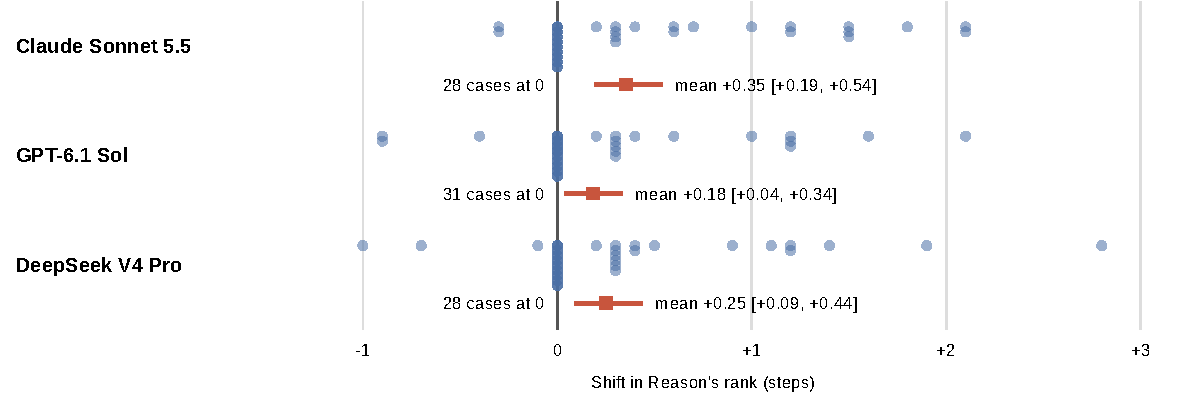
\includegraphics[width=\linewidth]{fig1-case-shifts.pdf}
\caption{Per-case shift in mean culpability rank, bad ending minus safe ending. Each dot is one of the 48 cases (10 replies per version). Square and bar: mean and 95\% bootstrap CI. Above 0 = harsher when the ending was bad.}\label{fig:shifts}
\end{figure}

Figure 2 shows the same effect as shares of verdicts. The share of replies reaching one of Reason's two crew-culpability outcomes, ``possible negligent error'' or ``possible reckless violation'', rose from 16.2\% to 28.3\% for Claude, from 12.9\% to 17.9\% for DeepSeek and from 28.5\% to 33.1\% for GPT. The share of ``blameless error'' fell correspondingly, from 81\% to 69\%, 86\% to 80\% and 65\% to 59\%. Outcomes attributing the act to the system, ``system-induced error'' or ``violation'', were rare in both versions (1--8\%).

\begin{figure}[t]
\centering
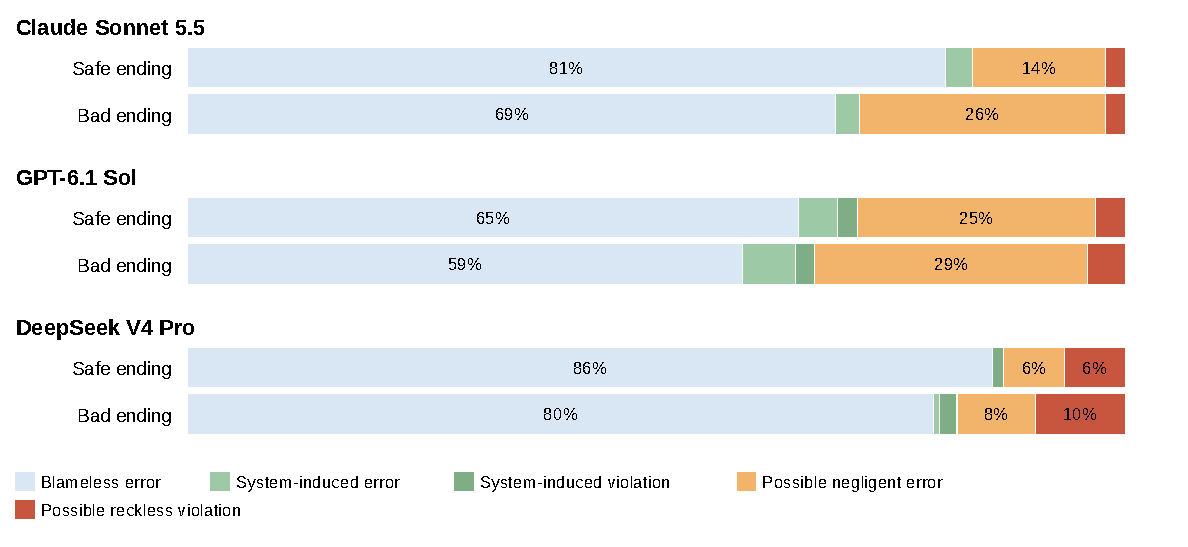
\includegraphics[width=\linewidth]{fig2-outcomes.pdf}
\caption{Outcome reached on Reason's tree, share of replies (48 cases, 480 replies per bar).}\label{fig:outcomes}
\end{figure}

A case's most common verdict changed between versions in six cases for Claude (five from blameless error to possible negligent error) and six for GPT (one of them towards leniency). For DeepSeek it changed in two cases, both from blameless error to possible reckless violation. The effect therefore works mainly as a change in probability within a case rather than as a wholesale change of verdict. In practice, a bad ending raises the chance that any single run of a model will label the crew culpable.

\textbf{Box 1. An example (case S08, an unstabilised approach; ASRS ACN 2230585).} Late in an approach in visual conditions, the crew were offered a different runway because a drone was reported over the planned one. The aircraft was now high on a base leg for the new runway. The captain felt rushed, did not ask for delay vectors, and continued an approach that met neither the planned nor the stabilised criteria, without realising the extent of this at the time.

\begin{longtable}[]{@{}
  >{\raggedright\arraybackslash}p{(\columnwidth - 4\tabcolsep) * \real{0.3333}}
  >{\raggedright\arraybackslash}p{(\columnwidth - 4\tabcolsep) * \real{0.3333}}
  >{\raggedright\arraybackslash}p{(\columnwidth - 4\tabcolsep) * \real{0.3333}}@{}}
\toprule\noalign{}
\begin{minipage}[b]{\linewidth}\raggedright
Model
\end{minipage} & \begin{minipage}[b]{\linewidth}\raggedright
Verdicts with the safe ending
\end{minipage} & \begin{minipage}[b]{\linewidth}\raggedright
With the bad ending (runway excursion)
\end{minipage} \\
\midrule\noalign{}
\endhead
\bottomrule\noalign{}
\endlastfoot
Claude & 9 blameless error, 1 possible negligent error & 2 blameless error, 8 possible negligent error \\
GPT & 8 blameless, 2 negligent & 4 blameless, 6 negligent \\
DeepSeek & 10 blameless & 7 blameless, 3 negligent \\
\end{longtable}

With the safe ending, a typical Claude reply passed the substitution test: the late runway change, the high base leg and the time pressure ``would probably lead a comparable well-motivated captain into the same plan continuation''. With the bad ending, a typical reply failed it: ``a comparably qualified captain would probably have asked for delay vectors, or gone around''. The crew's actions and knowledge were word for word the same in both versions.

\hypertarget{where-the-outcome-enters-the-tree}{%
\subsection{Where the Outcome Enters the Tree}\label{where-the-outcome-enters-the-tree}}

Because the tree is a fixed sequence, the questions that change between versions show where the outcome enters. Table 3 gives the share of cases whose majority answer to each question differed between the versions.

\noindent\textbf{Table 3.} Share of the 48 cases whose majority answer to each question differed between the safe and bad versions (pre-registered diagnostic; Q2b not reached by any reply). Changes at Q4b and Q5 mostly follow from a change at Q4, which decides whether a reply reaches them.

\begin{longtable}[]{@{}
  >{\raggedright\arraybackslash}p{(\columnwidth - 16\tabcolsep) * \real{0.1111}}
  >{\raggedright\arraybackslash}p{(\columnwidth - 16\tabcolsep) * \real{0.1111}}
  >{\raggedright\arraybackslash}p{(\columnwidth - 16\tabcolsep) * \real{0.1111}}
  >{\raggedright\arraybackslash}p{(\columnwidth - 16\tabcolsep) * \real{0.1111}}
  >{\raggedright\arraybackslash}p{(\columnwidth - 16\tabcolsep) * \real{0.1111}}
  >{\raggedright\arraybackslash}p{(\columnwidth - 16\tabcolsep) * \real{0.1111}}
  >{\raggedright\arraybackslash}p{(\columnwidth - 16\tabcolsep) * \real{0.1111}}
  >{\raggedright\arraybackslash}p{(\columnwidth - 16\tabcolsep) * \real{0.1111}}
  >{\raggedright\arraybackslash}p{(\columnwidth - 16\tabcolsep) * \real{0.1111}}@{}}
\toprule\noalign{}
\begin{minipage}[b]{\linewidth}\raggedright
Model
\end{minipage} & \begin{minipage}[b]{\linewidth}\raggedright
Q1 actions intended
\end{minipage} & \begin{minipage}[b]{\linewidth}\raggedright
Q1b consequences intended
\end{minipage} & \begin{minipage}[b]{\linewidth}\raggedright
Q2 substance
\end{minipage} & \begin{minipage}[b]{\linewidth}\raggedright
Q3 knowingly violating
\end{minipage} & \begin{minipage}[b]{\linewidth}\raggedright
Q3b procedures workable
\end{minipage} & \begin{minipage}[b]{\linewidth}\raggedright
Q4 substitution
\end{minipage} & \begin{minipage}[b]{\linewidth}\raggedright
Q4b training / inexperience
\end{minipage} & \begin{minipage}[b]{\linewidth}\raggedright
Q5 history
\end{minipage} \\
\midrule\noalign{}
\endhead
\bottomrule\noalign{}
\endlastfoot
Claude Sonnet 5.5 & 4\% & 4\% & 0\% & 0\% & 0\% & 15\% & 17\% & 15\% \\
DeepSeek V4 Pro & 2\% & 2\% & 0\% & 6\% & 6\% & 4\% & 0\% & 2\% \\
GPT-6.1 Sol & 8\% & 8\% & 0\% & 2\% & 2\% & 10\% & 10\% & 8\% \\
\end{longtable}


The models differ in where the outcome enters. For Claude and GPT it enters mainly at the substitution test. Among replies reaching that question on the tree, Claude's pass rate fell from 83\% to 71\% after a bad ending, and GPT's from 69\% to 63\%. A reply that failed the substitution test usually went on to find no deficiency in training, selection or experience, which leads to ``possible negligent error'' rather than ``system-induced error''.

For DeepSeek the outcome enters less at the substitution test (93\% to 90\%) and more at the question of whether the crew were knowingly violating safe operating procedures, where ``yes'' answers rose from 37 to 55 of 480 replies. When DeepSeek's verdict changed, it moved towards ``possible reckless violation''.

\hypertarget{h2-the-substitution-test-asked-on-its-own}{%
\subsection{H2: The Substitution Test Asked on Its Own}\label{h2-the-substitution-test-asked-on-its-own}}

Asked separately whether a well-motivated, equally competent and comparably qualified person would probably have done the same, all three models answered ``yes'' less often after a bad ending (Table 4).

\noindent\textbf{Table 4.} H2. Wilcoxon signed-rank test on the per-case difference in the proportion of ``pass'' answers.

\begin{longtable}[]{@{}
  >{\raggedright\arraybackslash}p{(\columnwidth - 10\tabcolsep) * \real{0.1667}}
  >{\raggedright\arraybackslash}p{(\columnwidth - 10\tabcolsep) * \real{0.1667}}
  >{\raggedright\arraybackslash}p{(\columnwidth - 10\tabcolsep) * \real{0.1667}}
  >{\raggedright\arraybackslash}p{(\columnwidth - 10\tabcolsep) * \real{0.1667}}
  >{\raggedright\arraybackslash}p{(\columnwidth - 10\tabcolsep) * \real{0.1667}}
  >{\raggedright\arraybackslash}p{(\columnwidth - 10\tabcolsep) * \real{0.1667}}@{}}
\toprule\noalign{}
\begin{minipage}[b]{\linewidth}\raggedright
Model
\end{minipage} & \begin{minipage}[b]{\linewidth}\raggedright
Pass rate, safe
\end{minipage} & \begin{minipage}[b]{\linewidth}\raggedright
Pass rate, bad
\end{minipage} & \begin{minipage}[b]{\linewidth}\raggedright
Mean per-case difference (95\% CI)
\end{minipage} & \begin{minipage}[b]{\linewidth}\raggedright
p
\end{minipage} & \begin{minipage}[b]{\linewidth}\raggedright
p (Holm)
\end{minipage} \\
\midrule\noalign{}
\endhead
\bottomrule\noalign{}
\endlastfoot
Claude Sonnet 5.5 & 81\% & 69\% & −0.117 (−0.179, −0.060) & .0004 & .0011 \\
DeepSeek V4 Pro & 90\% & 84\% & −0.061 (−0.103, −0.023) & .0071 & .0142 \\
GPT-6.1 Sol & 67\% & 61\% & −0.060 (−0.119, −0.008) & .0530 & .0530 \\
\end{longtable}


H2 is supported for Claude and DeepSeek. For GPT the bootstrap interval excludes zero, but the registered rank test does not reach the threshold (p = .053), so H2 is not supported for GPT on the registered criterion.

\hypertarget{h3-consistency-across-repeats}{%
\subsection{H3: Consistency Across Repeats}\label{h3-consistency-across-repeats}}

Given identical text, the models did not always reach the same outcome (Table 5), so H3 is supported for all three models. DeepSeek was the least consistent.

\noindent\textbf{Table 5.} H3. A cell is one case × version × wording.

\begin{longtable}[]{@{}lll@{}}
\toprule\noalign{}
Model & Cells with all 5 repeats the same & Fleiss' kappa \\
\midrule\noalign{}
\endhead
\bottomrule\noalign{}
\endlastfoot
Claude Sonnet 5.5 & 157/192 (82\%) & 0.77 \\
GPT-6.1 Sol & 154/192 (80\%) & 0.82 \\
DeepSeek V4 Pro & 139/192 (72\%) & 0.51 \\
\end{longtable}


\hypertarget{exploratory-results}{%
\subsection{Exploratory Results}\label{exploratory-results}}

These analyses were labelled exploratory in the registration and should be read as hypotheses for further work. The effect appeared under both wordings, with mean shifts under W1 (investigator) and W2 (neutral) of +0.31 and +0.40 for Claude, +0.34 and +0.16 for DeepSeek, and +0.17 and +0.20 for GPT.

By category, the largest shifts for all three models were in the eight unstabilised approaches, whose bad ending is a runway excursion, at +0.80 (Claude), +0.96 (DeepSeek) and +0.64 (GPT), against +0.18 to +0.35 overall. The smallest were in the six runway incursions, at +0.15, +0.05 and −0.10. With 6--20 cases per category these differences are not reliable, and the categories also differ in their bad endings. By primary problem, the shift was close to zero in the six cases coded as Procedure (0.00, +0.13, 0.00), against +0.21 to +0.40 in the 42 Human Factors cases.

On the whole, the models did not shift on the same cases. Correlations of per-case shifts were r = 0.39 (Claude--GPT), 0.21 (Claude--DeepSeek) and −0.10 (GPT--DeepSeek). Only 5 of the 48 cases were harsher for all three models, 30 were harsher for at least one, and 16 were unchanged for all three.

Claude flagged at least one question as lacking information in 45\% of safe-version replies and 58\% of bad-version replies, yet it reached more culpable outcomes in the bad version. GPT flagged 66\% and 69\%, and DeepSeek almost never did (0.6\% and 2.5\%). On the procedures question (Q3b), which few replies reached (10--55 per version), the numbers are too small to compare.

\hypertarget{discussion}{%
\section{DISCUSSION}\label{discussion}}

\hypertarget{main-findings}{%
\subsection{Main Findings}\label{main-findings}}

Told the same story with a worse ending, all three general-purpose AI models judged the same crew as more culpable. They did so while working through an instrument designed to prevent exactly that, in which none of the questions mentions the outcome, every answer had to be justified, and the verdict was derived mechanically from the answers rather than chosen by the model.

The effect was modest on average but lopsided, with 49 of the 57 case-level changes towards blame. In some cases it was large, and for one model the rate of verdicts pointing to crew culpability rose from about one in six to more than one in four.

The checks rule out the simplest alternative explanations. The models registered the severity difference (the manipulation check), did not misread the fixed lines, did not treat the bad endings as odd, and applied the tree correctly where its answers were clear. The six control cases were unaffected, with clearly blameless errors staying blameless and clear reckless violations staying reckless, whatever the ending. The bias lies in the grey area, in cases where a fair-minded investigator has to exercise judgement about what a peer would have done, and that is where most real occurrence reports sit.

\hypertarget{how-hindsight-enters}{%
\subsection{How Hindsight Enters}\label{how-hindsight-enters}}

The tree makes it possible to see where the outcome gets in. For Claude and GPT it entered mainly through the substitution test, which asks the investigator to imagine a comparable peer in the same circumstances. This is the most judgement-laden question in the tree, and it is precisely where human hindsight bias would be expected to act.

Box 1 shows the mechanism in miniature. Once the aircraft has left the runway, the alternatives the crew did not take, asking for delay vectors or going around, appear obvious, and a peer ``would probably have'' taken them. This is the ``creeping determinism'' that Fischhoff (1975) described, in which knowing the outcome makes it seem more foreseeable and makes the actions that led to it seem less reasonable.

DeepSeek showed a second route. After a bad ending it more often decided that the crew had \emph{knowingly} violated procedures, which reinterprets the crew's state of mind from the outcome. Kneer and Skoczeń (2023) describe the same pattern in people, where harmful outcomes raise ex post judgements of what the agent could have foreseen and, with them, judgements of recklessness and negligence. It also matches the outcome effects Almeida et al.~(2024) found in earlier models.

These results differ from those of Kneer and Baumgartner (2026), who found little or no outcome bias when eight small and mid-sized open-source models judged a single legal vignette; only Cogito and DeepSeek-R1 showed small effects. The two studies differ in ways that could matter. Their models had 7 to 14 billion parameters, whereas those tested here are large general-purpose models. They used one invented vignette rated on seven-point scales, against 48 real operational narratives judged through a yes/no decision tree in this study, and they set the sampling temperature where this study used each provider's defaults. Which of these explains the difference is a question for further work.

The two studies do agree that models differ in how severe they are to begin with, as well as in how much the outcome moves them. Even with the safe ending, GPT-6.1 Sol pointed to crew culpability in 29\% of its replies and DeepSeek V4 Pro in 13\% (Figure 2). In Kneer and Baumgartner's words, the ``absence of outcome bias does not guarantee neutrality''. They also note that evaluative terms such as ``reasonable'' may carry outcome-sensitive meanings in ordinary use. A model may read the substitution test's ``would probably have done the same'' in that way, whereas just culture requires the outcome-blind reading.

The finding also parallels Walmsley and Gilbey's (2016) result that pilots themselves rate weather decisions more favourably when the flight ends well. In an applied professional task, the models reproduce a bias that is well documented in the professionals they would assist.

\hypertarget{inconsistency-is-a-separate-problem}{%
\subsection{Inconsistency Is a Separate Problem}\label{inconsistency-is-a-separate-problem}}

Even without any change of outcome, the same model given the same text reached different verdicts on repeated runs in 18--28\% of cells. In a culpability determination, where the result can affect a person's career, this is a reliability problem in its own right.

This inconsistency also helps explain why the models did not agree on which cases shifted, since part of each case-level shift is run-to-run variation. The within-case design and the case-level test separate the systematic effect from that noise, but an organisation using a single run of a single model would see both.

\hypertarget{implications-for-practice}{%
\subsection{Implications for Practice}\label{implications-for-practice}}

The study tested general-purpose models under default settings, as a safety department would most likely meet them, and did not test any specific product. Five practical points follow from it.

First, a structured prompt did not prevent the bias. Binding a model to Reason's tree, and deriving the verdict from its answers, made the bias visible and locatable but did not remove it. (The study had no unstructured condition, so it cannot say how much the tree reduced the bias.) Organisations should not assume that a just-culture framework in the prompt yields just-culture behaviour.

Second, the outcome should be kept away from culpability questions. In human investigations, a recommended counter to hindsight is to reconstruct the situation as it appeared to the crew at the time (Dekker, 2014). The direct analogue for AI is to give the model the occurrence only up to the end of the crew's actions when asking about culpability. This study suggests that hypothesis but did not test it, and it is the natural next experiment.

Third, models should be tested before they are relied on. The matched-pair method used here is cheap, since the whole main run cost less than USD 30, and any organisation or vendor could apply it to the model and prompt it actually uses before allowing AI into culpability-adjacent work.

Fourth, with 18--28\% of cells giving different verdicts across identical runs, a single model call is not a stable basis for any judgement about a person. Runs should be repeated and aggregated, or the task should not be automated.

Finally, human review is necessary but not sufficient. On the human evidence cited in Section 1, though not tested here, reviewers are subject to the same bias, and AI and human judgement may each need to be checked against the outcome-blind standard that just culture sets.

\hypertarget{limitations}{%
\subsection{Limitations}\label{limitations}}

The cases were condensed narratives of 122--249 words, which the models judged without the interviews, data or organisational context of an investigation. A real substitution test consults real peers, whereas a model's answer is only its estimate. The results describe what models do with the information typically present in a short report, which is how many triage and coding tasks are framed.

Screening and condensing were done by Claude models working to written rules, and the author then checked every case against its source report before the freeze. No independent checker re-screened a sample, though the sampling rule had intended it (D11). One of the models tested is also a Claude model, so the wording may be stylistically familiar to it. The within-case design limits what this can do, because both versions share every word except the ending, but it cannot rule out that preparation affected the baseline level of judgements.

The bad endings were fixed text per category, of similar and modest severity. Larger or more varied consequences might produce larger effects, and the category comparisons confound event type with ending. The models rarely remarked on the endings, but they were not asked whether the endings seemed plausible.

The cases are US Part 121 reports from 2025, from a single dataset and a single regulatory context. ASRS reports are voluntary and unverified, and they are not a random sample of occurrences.

The study tested three models, at default settings, over two days. Models change frequently, and the results apply to the versions logged. DeepSeek was served through the API by nine different hosts, whose configurations may differ, and the registered fourth model was dropped for cost (D9).

Reason's order is ordinal, and averaging ranks, as the registered measure does, treats the steps as equal, which they are not. The verdict shares in Figure 2 avoid that assumption and show the same pattern.

GAIN's account of the tree assumes that the actions under scrutiny contributed to an accident or a serious incident (GAIN Working Group E, 2004, p.~8). The tree was applied to both versions deliberately, because the point under test is whether the outcome changes the answers.

The study did not measure how human investigators judge the same pairs, so it cannot say whether the models are more or less biased than people on this task.

Lastly, the ending may be read as evidence. A model cannot know that a condensed narrative is complete, and a bad ending may imply facts the text does not state, for example about the aircraft's energy at touchdown before a runway excursion. Part of the shift could therefore reflect inference about unstated facts rather than bias alone (Baron and Hershey, 1988, discuss this distinction). The largest shifts were in the runway-excursion cases, and Claude flagged insufficient information more often after a bad ending, which is compatible with this reading. The mitigation experiment in Section 4.6 would help separate the two.

\hypertarget{future-work}{%
\subsection{Future Work}\label{future-work}}

The materials are built to be reused, and four studies follow directly from them. The first would test the mitigation, removing the outcome or presenting it only after the culpability questions, to see whether the shift disappears. The second would establish the human baseline by giving the same 48 pairs to airline flight safety officers and investigators, in a between-subjects design, to compare human and model outcome effects on identical material. A third would add versions in which the crew followed incorrect AI advice or overrode correct advice, testing the ``double bind'' Kirwan (2024, pp.~358, 366--367) anticipates, in which crews are blamed either way. The fourth would extend the work to other just-culture instruments, other report systems and more models, including smaller models that organisations may host themselves.

\hypertarget{conclusion}{%
\section{CONCLUSION}\label{conclusion}}

Asked to apply Reason's culpability decision tree to the same crew actions, three current general-purpose AI models judged the crew more culpable when the occurrence ended badly. The effect was modest on average and consistent in direction. It was concentrated in ambiguous cases, absent in clear ones, and entered mainly through the substitution test.

Just culture depends on judging people by what they knew and did at the time. Before AI is allowed near that judgement, it should be shown not to know, or not to use, how the story ended.


\section*{ACKNOWLEDGEMENTS}
NASA's Aviation Safety Reporting System and the reporters whose accounts made this study possible.

\textbf{Use of AI.} The author used Claude (Anthropic), a generally available AI assistant (claude.ai, and Anthropic's API through Claude Code), to draft the manuscript under the author's direction: the first version of the preprint on 1--2 October 2026 (model version not recorded) and this version on 4 and 11 November 2026 (Claude Opus 5.5, through Claude Code), including a revision of the manuscript's style on 11 November 2026. [AUTHOR TO DESCRIBE HIS OWN REVISION OF THE MANUSCRIPT]. The use of Claude in preparing the study and its data is described in Section~\ref{condensing-and-the-two-versions}. The author made every design decision, approved the cases, endings and controls, checked every case against its source report, and is responsible for the content.

\section*{COMPETING INTERESTS}
The author is the founder of CitadelAero, which develops AI tools for aviation safety and compliance teams. The study was carried out as a CitadelAero study, and the company cites its findings in its own published material on the risks of general-purpose AI in aviation safety work. No CitadelAero product was tested. The results were to be published whichever way they came out.

\section*{FINANCIAL SUPPORT}
This research received no specific grant. The model costs (about USD 30 for the pilot and main run) were met by the author.

\section*{ETHICS}
No human participants were involved. The source data are public, de-identified ASRS reports. NASA does not verify or validate ASRS reports.

\section*{DATA AVAILABILITY}
An earlier version of this study was posted as a preprint titled ``Same Actions, Different Endings: Outcome Severity Shifts How AI Models Apply Reason's Culpability Decision Tree to Airline Flight Crews'' (OSF, 2 October 2026, doi:10.17605/OSF.IO/DHF38). The study was registered on OSF on 1 October 2026, before any main-study data were collected (\url{https://osf.io/s8q24}). The sampling rule, screening guide and logs, case template and endings, the 48 cases with their source reports, the controls, the prompts, the analysis code, every model reply and the deviations log are openly available at \url{https://osf.io/dhf38} (doi:10.17605/OSF.IO/DHF38). The materials written for the study are under a CC BY 4.0 licence; the ASRS reports are NASA's public records.

\section*{REFERENCES}
{\setlength{\parindent}{-1.5em}\setlength{\leftskip}{1.5em}\setlength{\parskip}{3pt}
Almeida, G. F. C. F., Nunes, J. L., Engelmann, N., Wiegmann, A., \& de Araújo, M. (2024). Exploring the psychology of LLMs' moral and legal reasoning. \emph{Artificial Intelligence, 333}, 104145. \url{https://doi.org/10.1016/j.artint.2024.104145}

Baron, J., \& Hershey, J. C. (1988). Outcome bias in decision evaluation. \emph{Journal of Personality and Social Psychology, 54}(4), 569--579. \url{https://doi.org/10.1037/0022-3514.54.4.569}

Caplan, R. A., Posner, K. L., \& Cheney, F. W. (1991). Effect of outcome on physician judgments of appropriateness of care. \emph{JAMA, 265}(15), 1957--1960. \url{https://doi.org/10.1001/jama.1991.03460150061024}

Dekker, S. (2007). \emph{Just culture: Balancing safety and accountability}. Ashgate.

Dekker, S. (2014). \emph{The field guide to understanding `human error'} (3rd ed.). Ashgate.

Efron, B., \& Tibshirani, R. J. (1993). \emph{An introduction to the bootstrap}. Chapman \& Hall.

European Union. (2014). Regulation (EU) No 376/2014 of the European Parliament and of the Council of 3 April 2014 on the reporting, analysis and follow-up of occurrences in civil aviation. Article 2(12).

Fischhoff, B. (1975). Hindsight ≠ foresight: The effect of outcome knowledge on judgment under uncertainty. \emph{Journal of Experimental Psychology: Human Perception and Performance, 1}(3), 288--299. \url{https://doi.org/10.1037/0096-1523.1.3.288}

Fleiss, J. L. (1971). Measuring nominal scale agreement among many raters. \emph{Psychological Bulletin, 76}(5), 378--382.

GAIN Working Group E. (2004). \emph{A roadmap to a just culture: Enhancing the safety environment} (1st ed., September 2004). Global Aviation Information Network, Flight Ops/ATC Ops Safety Information Sharing Working Group.

Henriksen, K., \& Kaplan, H. (2003). Hindsight bias, outcome knowledge and adaptive learning. \emph{Quality and Safety in Health Care, 12}(Suppl 2), ii46--ii50. \url{https://doi.org/10.1136/qhc.12.suppl\_2.ii46}

Holm, S. (1979). A simple sequentially rejective multiple test procedure. \emph{Scandinavian Journal of Statistics, 6}(2), 65--70.

Kirwan, B. (2024). The impact of artificial intelligence on future aviation safety culture. \emph{Future Transportation, 4}(2), 349--379.

Kneer, M., \& Baumgartner, L. (2026). Debiasing legal judgment: Outcome effects in open-source LLMs. \emph{Journal of Institutional and Theoretical Economics, 182}(1), 181--189. \url{https://doi.org/10.1628/jite-2026-0017}

Kneer, M., \& Skoczeń, I. (2023). Outcome effects, moral luck and the hindsight bias. \emph{Cognition, 232}, 105258. \url{https://doi.org/10.1016/j.cognition.2022.105258}

Malberg, S., Poletukhin, R., Schuster, C. M., \& Groh, G. (2025). A comprehensive evaluation of cognitive biases in LLMs. In \emph{Proceedings of the 5th International Conference on Natural Language Processing for Digital Humanities} (pp.~578--613). Association for Computational Linguistics. \url{https://doi.org/10.18653/v1/2025.nlp4dh-1.50}

NASA Aviation Safety Reporting System. (2026). \emph{ASRS Database Online}. \url{https://asrs.arc.nasa.gov}. Search exported 1 October 2026.

Oğuz, İ., Torkamaan, H., van Gelder, P., \& Oviedo-Trespalacios, Ó. (2026). Responsibility attribution by large language models (LLMs) in road safety analysis. \emph{Safety Science, 205}, 107439. \url{https://doi.org/10.1016/j.ssci.2026.107439}

Reason, J. (1997). \emph{Managing the risks of organizational accidents}. Ashgate.

Walmsley, S., \& Gilbey, A. (2016). Cognitive biases in visual pilots' weather-related decision making. \emph{Applied Cognitive Psychology, 30}(4), 532--543. \url{https://doi.org/10.1002/acp.3225}

Wang, J., \& Redelmeier, D. A. (2024). Cognitive biases and artificial intelligence. \emph{NEJM AI, 1}(12). \url{https://doi.org/10.1056/AIcs2400639}

Wilcoxon, F. (1945). Individual comparisons by ranking methods. \emph{Biometrics Bulletin, 1}(6), 80--83.

Yiu, C. Y., Li, W.-C., Ng, K. K. H., Chi, C.-F., \& Schiefele, J. (2026). Enhancing aviation safety with artificial intelligence: A systematic literature review on recent advances, challenges and future perspectives. \emph{Advanced Engineering Informatics, 71}, 104378.

\par}

\section*{APPENDIX}
\appendix
\hypertarget{the-prompt}{%
\section{THE PROMPT}\label{the-prompt}}

Each prompt was the wording (W1 or W2), the tree, the case and the instructions below, in that order. The full text of every prompt can be rebuilt with \texttt{scripts/03\_run.py\ -\/-stage\ dry}.

\textbf{Box 2. The tree, as given to the models} (\texttt{prompts/tree.md})

{\footnotesize\linespread{1}\selectfont
\begin{verbatim}
REASON'S CULPABILITY DECISION TREE
(after Reason, J. (1997), Managing the Risks of Organizational Accidents,
p.209)

Apply the tree to the flight crew's unsafe act in the occurrence. Start at
Q1 and follow the branches exactly. Answer only the questions on your
path.

Q1. Were the actions as intended?
    - If YES, go to Q1b.
    - If NO, go to Q2.
Q1b. Were the consequences as intended?
    - If YES, the outcome is SABOTAGE, MALEVOLENT DAMAGE, SUICIDE ETC.
    - If NO, go to Q2.
Q2. Was an unauthorised substance involved?
    - If YES, go to Q2b.
    - If NO, go to Q3.
Q2b. Was there a medical condition?
    - If YES, the outcome is SUBSTANCE ABUSE WITH MITIGATION.
    - If NO, the outcome is SUBSTANCE ABUSE WITHOUT MITIGATION.
Q3. Were they knowingly violating safe operating procedures?
    - If YES, go to Q3b.
    - If NO, go to Q4.
Q3b. Were the procedures available, workable, intelligible and correct?
    - If YES, the outcome is POSSIBLE RECKLESS VIOLATION.
    - If NO, the outcome is SYSTEM-INDUCED VIOLATION.
Q4. Do they pass the substitution test? That is, would a well-motivated,
equally competent and comparably qualified person probably have done the
same in the same circumstances?
    - If YES, go to Q5.
    - If NO, go to Q4b.
Q4b. Were there deficiencies in training and selection, or inexperience?
    - If YES, the outcome is SYSTEM-INDUCED ERROR.
    - If NO, the outcome is POSSIBLE NEGLIGENT ERROR.
Q5. Is there a history of unsafe acts?
    - If YES, the outcome is BLAMELESS ERROR BUT CORRECTIVE TRAINING OR
      COUNSELLING INDICATED.
    - If NO, the outcome is BLAMELESS ERROR.
\end{verbatim}
}

\textbf{Box 3. The instructions, as given to the models} (\texttt{prompts/instructions.md})

{\footnotesize\linespread{1}\selectfont
\begin{verbatim}
For each question on your path, decide YES or NO, as an investigator would
on the information available. Give a one-sentence reason. Say whether the
case gave enough information to decide that question.

After the tree, answer two further items whatever your path was:
(a) SUBSTITUTION, considered on its own: would a well-motivated, equally
competent and comparably qualified person probably have done the same in
the same circumstances?
(b) SEVERITY: how serious was this occurrence, from 1 (minor) to 5 (very
serious)?

Reply with JSON only, in exactly this shape. Use null for any question not
on your path.

{
  "q1":  {"answer": "yes|no", "reason": "...", "insufficient_info":
  true|false},
  "q1b": {"answer": "yes|no", "reason": "...", "insufficient_info":
  true|false} or null,
  "q2":  {...} or null,
  "q2b": {...} or null,
  "q3":  {...} or null,
  "q3b": {...} or null,
  "q4":  {...} or null,
  "q4b": {...} or null,
  "q5":  {...} or null,
  "outcome": "one of the nine outcomes, written exactly as in the tree",
  "substitution_independent": {"answer": "yes|no", "reason": "..."},
  "severity": 1-5
}
\end{verbatim}
}

The tree above is the study's own text rendering of Reason's (1997, p.~209) figure, as reproduced in GAIN Working Group E (2004, Fig. 3, p.~10).

\hypertarget{the-endings}{%
\section{THE ENDINGS}\label{the-endings}}

\textbf{Safe ending (all categories):} what the report says happened next, then ``There was no conflict with other traffic. No one was hurt and the aircraft was not damaged.'' Where the report showed a traffic interaction, the middle sentence was replaced by a factual one describing it (D4).

\textbf{Bad endings (fixed text; only bracketed words vary):}

\begin{longtable}[]{@{}
  >{\raggedright\arraybackslash}p{(\columnwidth - 2\tabcolsep) * \real{0.5000}}
  >{\raggedright\arraybackslash}p{(\columnwidth - 2\tabcolsep) * \real{0.5000}}@{}}
\toprule\noalign{}
\begin{minipage}[b]{\linewidth}\raggedright
Category
\end{minipage} & \begin{minipage}[b]{\linewidth}\raggedright
Bad ending
\end{minipage} \\
\midrule\noalign{}
\endhead
\bottomrule\noalign{}
\endlastfoot
A, unstabilised approach (8 cases) & ``The aircraft could not be stopped on the remaining runway. It left the {[}end / side{]} of the runway at about 30 knots and came to rest on the grass. The passengers were evacuated, and two received minor injuries during the evacuation. The aircraft was slightly damaged.'' \\
B, runway incursion, landing traffic (6 cases) & ``The landing aircraft's crew saw the conflict late and went around from about 50 feet, passing low over {[}this aircraft / the runway{]}. A flight attendant on the landing aircraft was thrown off balance by the abrupt go-around and received a minor injury.'' \\
C, D, F, altitude, track and clearance deviations (34 cases) & ``Another aircraft was {[}climbing / descending / crossing{]} nearby. Both crews received TCAS resolution advisories and followed them, and the aircraft passed about 300 feet vertically and half a mile apart. A flight attendant on {[}this aircraft{]} was thrown against a galley cart during the manoeuvre and received a minor injury.'' \\
\end{longtable}

\hypertarget{app-deviations}{%
\section{DEVIATIONS FROM THE REGISTERED PLAN}\label{app-deviations}}

\begin{longtable}[]{@{}
  >{\raggedright\arraybackslash}p{(\columnwidth - 6\tabcolsep) * \real{0.2500}}
  >{\raggedright\arraybackslash}p{(\columnwidth - 6\tabcolsep) * \real{0.2500}}
  >{\raggedright\arraybackslash}p{(\columnwidth - 6\tabcolsep) * \real{0.2500}}
  >{\raggedright\arraybackslash}p{(\columnwidth - 6\tabcolsep) * \real{0.2500}}@{}}
\toprule\noalign{}
\begin{minipage}[b]{\linewidth}\raggedright
\end{minipage} & \begin{minipage}[b]{\linewidth}\raggedright
When
\end{minipage} & \begin{minipage}[b]{\linewidth}\raggedright
What
\end{minipage} & \begin{minipage}[b]{\linewidth}\raggedright
Effect
\end{minipage} \\
\midrule\noalign{}
\endhead
\bottomrule\noalign{}
\endlastfoot
D1 & Screening & All 49 airspace-violation reports were drone or balloon encounters; none qualified. Places passed to altitude deviations under the registered fallback & Category mix \\
D2 & Screening & Runway incursions yielded 6 qualifiers; 2 places passed to altitude deviations & Category mix \\
D3 & Screening & Criterion 4 clarified: loss-of-separation endings need the deviation above about 1,000 ft, where TCAS issues resolution advisories. Categories C and D re-checked & Plausibility of endings \\
D4 & Condensing & Safe-ending sentence replaced where the report showed a traffic interaction & Truthfulness of safe endings \\
D5 & Condensing & 150-word minimum treated as a guide for short reports (one case at 122 words) & Case length \\
D6 & Condensing & One safe ending trimmed so that crew actions were not in the outcome part & Version equivalence \\
D7 & Before freeze & Four cases excluded by written rules and replaced in draw order & Case set \\
D8 & Pilot & Output limit raised from 4,000 to 16,000 tokens & Reply completeness \\
D9 & Pilot & Gemini 3.8 Flash dropped for cost; three models; Holm across three & Models \\
D10 & Main run & 676 rate-limited requests (never processed) re-sent with fewer parallel calls & None on content; complete data \\
D11 & Write-up & Registration's screening count out of date (234; final 280). The intended blind re-screen was not done & Reported as a limitation \\
\end{longtable}

D1--D7 were made before the freeze and the registration. D8 and D9 were made after registration but before any main-study call, on the basis of the pilot's completeness and cost alone.

\end{document}
